\section{Farb- nach Grau-Bild}
Da die Berechnungen von ElSe auf Grau-Bildern arbeitet und das Eingabebild in Farbe ist, muss es in ein Grau-Bild umgewandelt werden. Dabei soll vor allem der Farbunterschied zwischen Pupille und der Umgebung maximal sein.\\
Die Problematik bei der Wahl des Verfahrens liegt in der Anforderung, da die Pupille möglichst dunkel sein soll und das restliche Auge hell. Die Farbe der Iris erschwert die Differenzierung da, wenn sie recht dunkel ist, der Grau-Wert zur Pupille entsprechend gering ist. Andererseits, ist das erkennen der Pupille bei sehr kleinen Bildern schwierig bis unmöglich wodurch auf der Iris gerechnet werden muss, und daher diese weiterhin erhalten bleiben muss.\\
Um die Auswirkung der verschiedenen Farb- nach Grau-Bilder Konverter zu  ermitteln wurden einige Verfahren verwendet um ihre Auswirkung auf die Detektion zu ermitteln. Nach der Umwandlung von Farb- nach Grauwert wird für die Anwendung das Grau-Bild noch normiert, damit Mindestens ein schwarzes und ein weißes Pixel vorhanden ist.
\begin{figure}
	\centering
	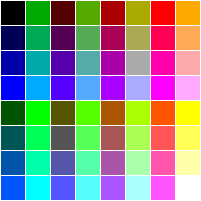
\includegraphics[width=0.2\linewidth]{img/Farbtafel2}
	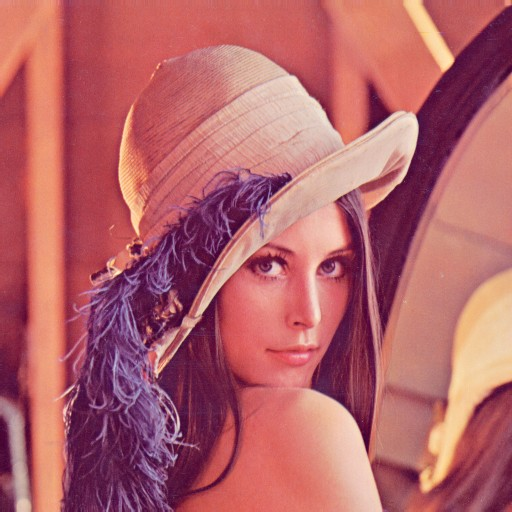
\includegraphics[width=0.2\linewidth]{img/lena}
	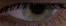
\includegraphics[width=0.2\linewidth]{img/Auge}
	\caption{Dies sind die Eingabebilder der verschiedenen Konverter von Farbe nach Grau. Links eine Farbpalette, Mittel Lena und Rechts ein Augenausschnitt aus dem Augendatensatz \cite{database_Eye}}
	\label{img_Gray_Einagbe}
\end{figure}
\subsection{Luminance}
\label{gray_Luminance}
Dies ist ein lineares Verfahren, das der menschlichen Farbwahrnehmung entspricht. Eine Gamma-Korrektur wird bei der Umwandlung nicht verwendet, siehe \autoref{img_Luminance}.\\
Somit entsteht ein natürlicher Farbverlauf, bei dem der Farbunterschied zwischen Pupille, Iris und Auge auf einem mittleren Niveau bleibt. Außerdem ist dieses Verfahren oft Standard bei der Umwandlung von Farb- nach Grau-Bilder.
\[G_{Luminance} = 0.299 \cdot R + 0.587 \cdot G + 0.114 \cdot B\]
\begin{figure}
	\centering
	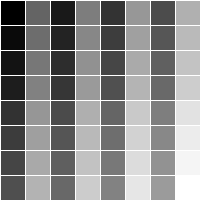
\includegraphics[width=0.2\linewidth]{img/Farbkarte_Normal}
	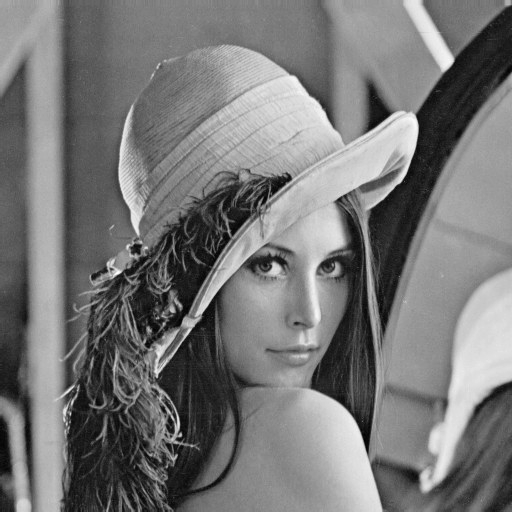
\includegraphics[width=0.2\linewidth]{img/Lena_Normal}
	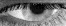
\includegraphics[width=0.2\linewidth]{img/Auge_NormGray}
	\caption{Ergebnis der Umwandlung von Farb- nach Grauwert mittels Luminance-Verfahren}
	\label{img_Luminance}
\end{figure}
\subsection{Gleam}
\label{gray_Gleam}
Bei dem Gleam Verfahren wird jede Farbe (Rot,Gelb und Grün) gleich stark bewertet allerdings wird jeder Farbwert mittels einer Gamma-Korrektur verbessert und das Bild wirkt heller als bei dem Luminance-Verfahren, siehe \autoref{img_Gleam}.\\
Durch die Gamma-Korrektur wird vor allem der helle Bereich weiter erhöht, somit wird der Farbunterschied zwischen Iris und Auge vermindert, wodurch die Pupille der einzige dunkle Bereich wird.\\
Allerdings wird auch dieser Farbwert erhöht und, sollte die Pupille nicht schwarz sein, nur noch ein grauer Bereich vorhanden ist.\\
Dieses Verfahren wurde gewählt, da es im Vergleich zu den anderen Verfahren von \glqq Color-to-Grayscale: Does the Method Matter in Image Recognition?\grqq \cite{rgb_to_Gray} am besten abgeschnitten hat.
\[G_{Gleam}=\dfrac{R^{\frac{1}{2.2}} + G^{\frac{1}{2.2}} + B^{\frac{1}{2.2}}}{3}\]
\begin{figure}
	\centering
	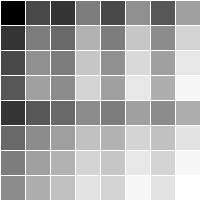
\includegraphics[width=0.2\linewidth]{img/Farbkarte_22}
	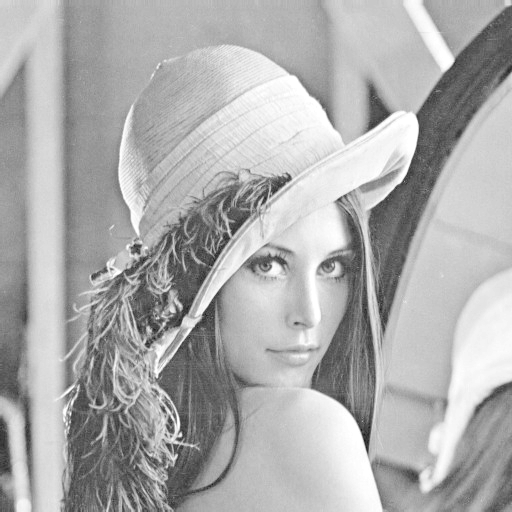
\includegraphics[width=0.2\linewidth]{img/Lena_22}
	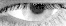
\includegraphics[width=0.2\linewidth]{img/Auge_22Gray}
	\caption{Ergebnis der Umwandlung von Farb- nach Grauwert mittels Glean-Verfahren}
	\label{img_Gleam}
\end{figure}
\subsection{Gleam-New}
\label{gray_New}
Dies ist eine verbesserte Variante von Gleam bei dem zuerst das gesamte Bild analysiert wird um die Parameter für die jeweilige Gamma-Korrektur zu ermitteln.\\
Durch die individuelle Veränderung der Farbkanäle, werden Farbunterschiede minimiert und somit alle stark farbigen Bereiche ebenfalls dunkel dargestellt. Somit wird der Kontrast zwischen der farbigen Iris und dem weißen Auge verbessert, siehe \autoref{img_NewGeam}.\\
Da allerdings alle Farben dunkel werden, entstehen weitere dunkle Bereiche die die Detektion der Pupille beeinträchtigen können. Ein kleiner Nachteil ist die vorige Analyse des Bildes um die Parameter entsprechend passend wählen zu können
\[G_{Gleam New}=\dfrac{R^{r} + G^{g} + B^{b}}{3}\]
Wobei gilt $\{r,g,b\} = \frac{\log(V_{\max})}{\log(\{R,G,B\}_{\max})}$ mit $V_{\max}$ als maximal möglicher Farbwert und $R_{\max}$ als maximal Vorhandener Rot-Farbwert, $G_{\max}$ und $B_{\max}$ äquivalent.
\begin{figure}
	\centering
	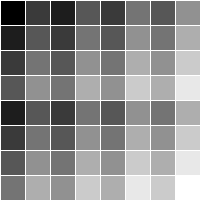
\includegraphics[width=0.2\linewidth]{img/Farbkarte_New}
	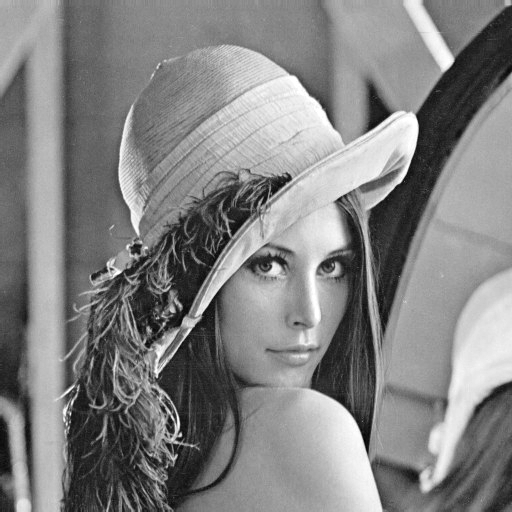
\includegraphics[width=0.2\linewidth]{img/Lena_New}
	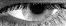
\includegraphics[width=0.2\linewidth]{img/Auge_NewGray}
	\caption{Ergebnis der Umwandlung von Farb- nach Grauwert mittels Gleam-New-Verfahren}
	\label{img_NewGeam}
\end{figure}
\subsection{Quadrat}
\label{gray_Quadrat}
Dies ist ein Verfahren, dass das Eingabebild verdunkelt und vom Aufbau dem Inversen von Gleam entspricht. Somit ist das gesamte Bild dunkler als bei dem Luminance-Verfahren, siehe \autoref{img_Quadrat}.
Durch die Abdunklung werden kleine Farbänderungen in den dunklen Bereichen reduziert, wodurch die Pupille klarer zu sehen sein sollte, der Farbunterschied zur Iris allerdings ebenfalls verringert wird.
\[G_{Quadrat}=\dfrac{R^2+G^2+B^2}{3}\]
\begin{figure}
	\centering
	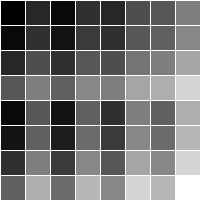
\includegraphics[width=0.2\linewidth]{img/Farbkarte_Quadrat}
	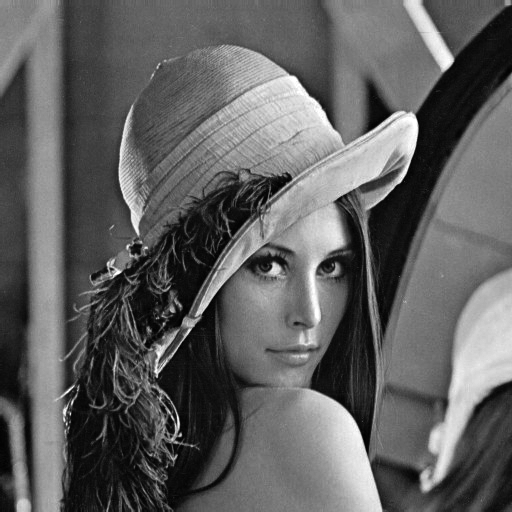
\includegraphics[width=0.2\linewidth]{img/Lena_Quadrat}
	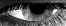
\includegraphics[width=0.2\linewidth]{img/Auge_QuadratGray}
	\caption{Ergebnis der Umwandlung von Farb- nach Grauwert mittels Quadrat-Verfahren}
	\label{img_Quadrat}
\end{figure}
\subsection{Min-Max-Verfahren}
\label{gray_MinMax}
Dabei handelt es sich eigentlich um zwei verschiedene Varianten, allerdings funktionieren beide nach dem selben Prinzip, als Grauwert wird der jeweilige Extremwert aus den Farben gewählt.\\
Durch Verwendung der Extremwerte, wird das gesamte Bild deutlich heller bzw. dunkler und kleinere Farbänderungen werden entfernt.\\
Bei dem Max-Verfahren werden alle farbigen und helle Bereiche bleiben Hell und nur gleichmäßig dunkel Bereiche bleiben dunkel wie es bei schwarz der Fall ist.\\
Wenn der Minimalwert anstelle verwendet wird, bleiben nur gleichmäßig helle Bereiche hell, alles andre wird abgedunkelt.
\begin{align*}
G_{max} &= \max(R,G,B)\\
G_{min} &= \min(R,G,B)
\end{align*}
\begin{figure}
	\centering
	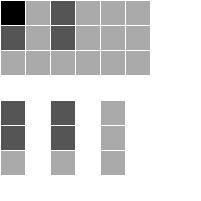
\includegraphics[width=0.2\linewidth]{img/Farbkarte_Max}
	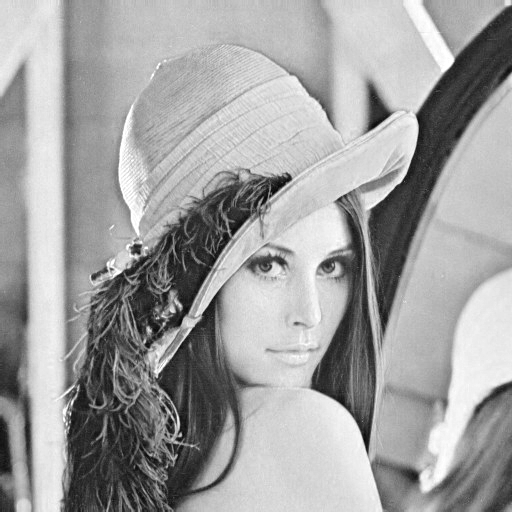
\includegraphics[width=0.2\linewidth]{img/Lena_Max}
	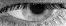
\includegraphics[width=0.2\linewidth]{img/Auge_MaxGray}\\
	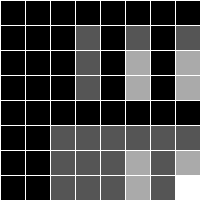
\includegraphics[width=0.2\linewidth]{img/Farbkarte_Min}
	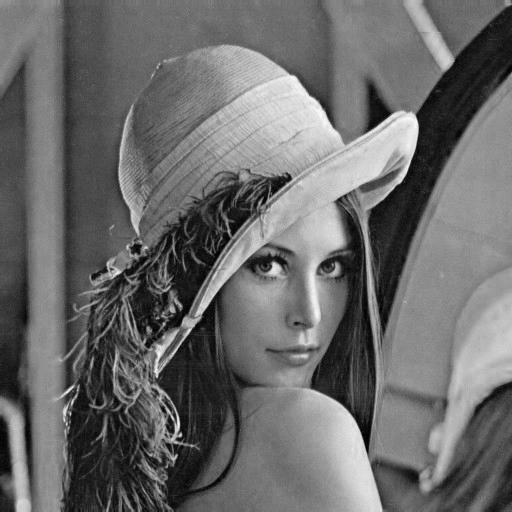
\includegraphics[width=0.2\linewidth]{img/Lena_Min}
	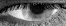
\includegraphics[width=0.2\linewidth]{img/Auge_MinGray}
	\caption{Ergebnis der Umwandlung von Farb- nach Grauwert mittels Extremwert-Verfahren. Oben: Max-Verfahren, Unten: Min-Verfahren}
	\label{img_MinMax}
\end{figure}
\subsection{Normalisierung von Graubilder}
Um ein Graubild zu erhalten, dass das volle Spektrum der möglichen Werte erfüllt, wird das Eingabebild normalisiert. Dazu wird der Maximale $G_{max}$ und Minimale $G_{min}$ im Bild gesucht um anschließend wird der neue Grau-Wert $G_{new}$ wie folgt bestimmt, dabei ist $V_{max}$ der maximal größte Wert.
\[G_{new} = G\cdot \dfrac{V_{max}+G_{min}}{G_{max}}-G_{min}\]
Da für die Anwendung ein Schwarzer Bereich gesucht wird gegen einen Hellen Hintergrund, wird für die Bestimmung der Extremwerte nicht das originale Eingenbild verwendet, sonder ein Gauß-gefiltertes.\\
Dies hat den Vorteil, das einzelne lokal auftretende Werte nicht verwendet werden als Extremwert. Mit dem Ergebnis, dass die Pupille gleichmäßiger dunkler wird und Pixel die eine Reflektion darstellen ignoriert werden und somit das gesamte Bild stärker aufgehellt wird.a